\documentclass[conference]{IEEEtran}

\usepackage{amsmath,amssymb,amsfonts}
\usepackage{graphicx}
\usepackage{textcomp}
\usepackage{xcolor}
\usepackage{booktabs}
\usepackage{multirow}
\usepackage{pgfplots}
\usepackage{pgfplotstable}
\usepackage{tikz}
\usepackage{hyperref}
\usepackage{algorithm}
\usepackage{algpseudocode}
\usepackage{subcaption}
\usepackage{balance}

\pgfplotsset{compat=1.18}

\definecolor{phase2color}{HTML}{2196F3}
\definecolor{tool1color}{HTML}{4CAF50}
\definecolor{tool2color}{HTML}{FF9800}
\definecolor{bothcolor}{HTML}{9C27B0}
\definecolor{hardnoisecolor}{HTML}{F44336}
\definecolor{softnoisecolor}{HTML}{009688}

\begin{document}

\title{Extending TICODER with Soft Scoring and Entropy-Based Early Stopping for Robust Interactive Code Generation}

\author{
\IEEEauthorblockN{Noori}
\IEEEauthorblockA{
\textit{Software Engineering} \\
}
}

\maketitle

\begin{abstract}
We reproduce TICODER, a test-driven interactive code generation framework, on the MBPP benchmark (427 tasks) using Claude Haiku and extend it with an integrated feedback loop comprising soft scoring and entropy-based early stopping. Soft scoring replaces TICODER's irreversible hard pruning with cumulative agreement scores ($+1$/$-1$), keeping all candidates alive; entropy-based stopping monitors behavioral convergence after each oracle response and terminates when further interactions would not change the ranking. Together, these form a natural cycle: the discriminative metric selects the most informative test, the oracle answers, soft scoring accumulates the evidence, and entropy checks whether the uncertainty has been resolved. This combined approach improves \textsc{PassFail} accuracy by +1.63 percentage points over hard pruning while using 54\% fewer oracle calls. Its primary value emerges under noise: when 1 in 5 oracle responses is incorrect, hard pruning suffers a permanent $-6.09$ point degradation, whereas soft scoring limits the damage to $-1.17$ points and self-recovers by the third interaction, offering a practical path toward deploying interactive code generation with imperfect feedback signals.
\end{abstract}

\begin{IEEEkeywords}
code generation, test-driven development, large language models, interactive systems, noise robustness
\end{IEEEkeywords}

% ============================================================
\section{Introduction}
% ============================================================

Large language models (LLMs) have demonstrated remarkable capabilities in automated code generation~\cite{chen2021codex, li2023starcoder, roziere2023codellama}, with recent models achieving substantial pass rates on standard benchmarks. However, a fundamental challenge remains: when a model generates multiple candidate solutions, how do we reliably select the correct one?

The standard approach of sampling $k$ candidates and reporting pass@$k$~\cite{chen2021codex} sidesteps the selection problem entirely. In practice, a developer must choose \emph{one} solution to integrate into their codebase. Random selection yields pass@1, which is typically far below pass@$k$, leaving significant potential unrealized.

TICODER~\cite{ticoder} introduced a promising solution through interactive test-driven refinement. By generating both code and test suggestions, then iteratively querying an oracle (e.g., a developer or reference implementation) about test correctness, TICODER progressively eliminates incorrect candidates through \emph{hard pruning}. This approach has been shown to substantially improve selection quality, effectively bridging the gap between pass@1 and pass@$k$.

However, TICODER's design makes two assumptions that limit practical deployment:

\begin{enumerate}
    \item \textbf{Fixed interaction budget.} Every task receives the same number of oracle interactions ($m=5$), regardless of whether the candidates converged after the first query. In scenarios where oracle calls are expensive---such as human code review or execution in sandboxed environments---this wastes resources on tasks that are already resolved.
    \item \textbf{Perfect oracle.} Hard pruning permanently removes any code that disagrees with the oracle on a single test. This is optimal when the oracle is always correct, but catastrophic when it is not. A single incorrect oracle response can irreversibly eliminate the correct solution.
\end{enumerate}

In this work, we reproduce TICODER on the MBPP benchmark~\cite{austin2021mbpp} using Claude Haiku and introduce an integrated extension that addresses both limitations through a unified feedback loop:

\begin{itemize}
    \item \textbf{Soft Scoring} replaces irreversible hard pruning with cumulative evidence accumulation. Each oracle interaction adjusts a code's score by $+1$ (agreement) or $-1$ (disagreement), but never removes it. This enables recovery from incorrect oracle signals through subsequent correct interactions.
    \item \textbf{Entropy-Based Early Stopping} monitors the behavioral diversity of code suggestions after each soft scoring update using Shannon entropy over execution-based clusters. When diversity collapses below a threshold, the loop terminates early.
\end{itemize}

These two mechanisms are deeply coupled: entropy-based stopping is only meaningful with soft scoring. Under hard pruning, all surviving codes agree on approved tests \emph{by construction} (disagreeing codes were eliminated), making entropy trivially zero after the first interaction. With soft scoring, no codes are removed, so entropy reflects genuine behavioral diversity and provides a principled stopping criterion.

We evaluate this approach through a four-phase experimental design, culminating in a controlled noise robustness study that quantifies the practical benefits under imperfect oracle conditions.

Our contributions are:
\begin{itemize}
    \item A faithful reproduction of TICODER on MBPP with Claude Haiku, establishing reference scores for the \textsc{PassFail} and \textsc{Output} oracle variants.
    \item An integrated soft scoring and entropy-based stopping loop that improves \textsc{PassFail} accuracy by +1.63 points while using 54\% fewer oracle calls.
    \item A controlled noise robustness experiment showing that soft scoring limits accuracy loss to 1.17 points under 20\% noise, compared to 6.09 points for hard pruning.
\end{itemize}

% ============================================================
\section{Background and Related Work}
% ============================================================

\subsection{Code Generation with LLMs}

The emergence of large language models trained on code~\cite{chen2021codex, li2023starcoder, roziere2023codellama} has transformed automated programming. Given a natural language description of a desired function, these models generate candidate implementations by sampling from the model's output distribution. Higher temperatures and multiple samples increase the likelihood of producing at least one correct solution, captured by the pass@$k$ metric~\cite{chen2021codex}:

\begin{equation}
    \text{pass@}k = \mathbb{E}_{\text{problems}} \left[ 1 - \frac{\binom{n-c}{k}}{\binom{n}{k}} \right]
\end{equation}

where $n$ is the total number of generated samples and $c$ is the number of correct ones. While pass@$k$ with large $k$ can be high, practical deployment requires selecting a single solution (pass@1), motivating work on candidate selection and ranking.

\subsection{Test-Based Selection Methods}

Several approaches leverage generated tests for candidate selection. \textbf{CodeT}~\cite{chen2022codet} generates test cases alongside code, then selects the candidate that passes the most generated tests. This ``consensus'' approach treats each test as a vote---codes that agree with more tests are more likely to be correct. \textbf{MBR-Exec}~\cite{shi2022mbr} applies minimum Bayes risk decoding using execution agreement, selecting the candidate whose outputs most closely match the majority.

These methods are non-interactive: they use all generated tests in a single batch. TICODER extends this paradigm by introducing \emph{iterative interaction} with an oracle, enabling progressive refinement.

\subsection{TICODER: Interactive Code Selection}

TICODER~\cite{ticoder} formulates code selection as an interactive process with four key components:

\textbf{Generation.} Given a task description and function header, the LLM generates $N$ code suggestions and $T$ test suggestions independently.

\textbf{Execution Matrix.} Each code is executed against each test, producing a matrix of pass/fail/crash results. This matrix is computed once and reused across all interactions.

\textbf{Discriminative Test Ranking.} At each interaction step, TICODER selects the test that maximally splits surviving candidates. Let $U$ be the set of test suggestions and $G$ be the set of code suggestions that have not been pruned away after $k \geq 0$ user interactions. For each test $t \in U$, the set $G$ is split into $G_t^+$ and $G_t^-$---the codes that pass and fail the assertion in $t$, respectively. Codes that crash are treated as precondition violations and ignored. Tests are ranked in decreasing order using the discriminative scoring metric:

\begin{equation}
    s_{\text{discr}}(t) = \begin{cases}
        0 & \text{if } \max(|G_t^+|, |G_t^-|) = 0, \\[4pt]
        \dfrac{\min(|G_t^+|, |G_t^-|)}{\max(|G_t^+|, |G_t^-|)} & \text{otherwise.}
    \end{cases}
    \label{eq:sdiscr}
\end{equation}

Tests with $s_{\text{discr}}$ close to 1 split the surviving codes most evenly and are therefore shown to the oracle first, as they prune the most candidates regardless of the oracle's response.

\textbf{Hard Pruning.} After querying the oracle about the selected test, TICODER permanently removes codes that disagree with the oracle's response. For \textsc{PassFail}, if the oracle says PASS, codes that fail the test are removed; if FAIL, codes that pass are removed. The \textsc{Output} variant provides the correct output value on failure, enabling even stricter pruning.

\textbf{Code Ranking.} Each surviving code $c \in G$ is executed against each used test $t \in U$ and receives a discriminative coverage score $d_c$ equal to the number of passing tests. Codes are ranked in decreasing order of $d_c$.

TICODER introduces the pass@$k$@$m$ metric to evaluate selection quality as a function of the number of oracle interactions $m$. Unlike pass@$k$, which is a statistical measure over random samples, pass@$k$@$m$ deterministically checks whether any of the top-$k$ ranked code suggestions (after $m$ interactions) is correct:

\begin{equation}
    \text{pass@}k\text{@}m = \mathbb{E}_{\text{problems}} \left[ \mathbf{1}[\text{any top-}k \text{ code after } m \text{ interactions is correct}] \right]
\end{equation}

\subsection{Running Example}

To illustrate the TICODER workflow, consider an MBPP task: \emph{``Write a function to check if a string contains sequences of lowercase letters joined with an underscore.''}  Suppose the LLM generates three code suggestions $c_1, c_2, c_3$ and three test suggestions $t_1, t_2, t_3$:

\begin{small}
\begin{verbatim}
  t1: assert func("aab_ccc_ddd") == True
  t2: assert func("aa_bb")       == True
  t3: assert func("AA_bb")       == False
\end{verbatim}
\end{small}

The execution matrix shows which codes pass each test:

\begin{table}[h]
\centering
\begin{small}
\begin{tabular}{lccc}
\toprule
 & $c_1$ & $c_2$ & $c_3$ \\
\midrule
$t_1$: \texttt{"aab\_ccc\_ddd"} & \textcolor{green!60!black}{pass} & \textcolor{red}{fail} & \textcolor{red}{fail} \\
$t_2$: \texttt{"aa\_bb"} & \textcolor{green!60!black}{pass} & \textcolor{green!60!black}{pass} & \textcolor{red}{fail} \\
$t_3$: \texttt{"AA\_bb"} & \textcolor{green!60!black}{pass} & \textcolor{green!60!black}{pass} & \textcolor{green!60!black}{pass} \\
\bottomrule
\end{tabular}
\end{small}
\end{table}

The discriminative scores are: $s_{\text{discr}}(t_1) = \min(1,2)/\max(1,2) = 1/2$, $s_{\text{discr}}(t_2) = \min(2,1)/\max(2,1) = 1/2$, and $s_{\text{discr}}(t_3) = 0/3 = 0$. Tests $t_1$ and $t_2$ tie with the highest score and are presented first. If the oracle responds FAIL for $t_1$ (the correct answer, since the function should only accept two segments joined by one underscore), TICODER prunes $c_1$ (which passed the test). After this interaction, $c_3$---the correct implementation---can rise to the top of the ranking.

This example illustrates both the power and fragility of hard pruning: if the oracle had \emph{incorrectly} responded PASS for $t_1$, the correct codes $c_2$ and $c_3$ would have been permanently eliminated instead.

\subsection{Limitations of Hard Pruning Under Noise}

The paper notes that TICODER assumes a \emph{faithful} oracle that always provides correct responses. In practice, oracles may be noisy: human annotators make mistakes, test specifications can be ambiguous, and flaky tests may produce inconsistent results. Hard pruning offers no mechanism to recover from such errors---once a correct code is pruned due to a noisy oracle response, it cannot be restored. This motivates our soft scoring extension, which treats oracle responses as \emph{evidence} rather than \emph{verdicts}.

% ============================================================
\section{Methodology}
% ============================================================

\subsection{Experimental Setup}

We use the following fixed settings across all experiments:

\begin{itemize}
    \item \textbf{Model:} Claude Haiku (\texttt{claude-haiku-4-5})
    \item \textbf{Dataset:} MBPP~\cite{austin2021mbpp}, sanitized split (427 tasks)
    \item \textbf{Code suggestions:} $N = 100$ per task
    \item \textbf{Test suggestions:} $T = 50$ per task
    \item \textbf{Max interactions:} $m = 5$
    \item \textbf{Temperature:} 0.8
    \item \textbf{Oracle:} Reference solution (simulated perfect oracle for Phases 2--3)
\end{itemize}

All LLM generations are cached after Phase~2. Phases 3 and 4 reuse these cached generations, ensuring that any differences in results are attributable solely to the selection algorithm, not to generation variance. This cache-and-reuse design eliminates a major source of experimental noise.

\subsection{An Integrated Feedback Loop: Soft Scoring with Entropy-Based Early Stopping}

Our extensions address two complementary limitations of TICODER. Rather than independent tools, they form a single coherent feedback loop in which each component plays a specific role:

\begin{enumerate}
    \item \textbf{$s_{\text{discr}}$ picks the most informative question.} The discriminative scoring metric (Eq.~\ref{eq:sdiscr}) selects the test that splits codes most evenly, maximizing the information gained from the oracle's response.
    \item \textbf{Soft scoring accumulates the oracle's answer as evidence.} Instead of permanently pruning codes, each oracle response adjusts every code's cumulative score by $+1$ (agreement) or $-1$ (disagreement). No code is ever removed.
    \item \textbf{Entropy measures whether the answer resolved the uncertainty.} After updating scores, we check whether codes have converged to a single dominant behavior. If so, further questions are unlikely to change the ranking, and we stop early.
\end{enumerate}

This loop continues until entropy drops below a threshold or the interaction budget is exhausted. Crucially, entropy-based stopping is only meaningful with soft scoring: under hard pruning, all surviving codes agree on every approved test \emph{by construction} (disagreeing codes were already eliminated), so entropy is trivially zero after the first approval. With soft scoring, all codes remain in the pool, and entropy provides a genuine measure of behavioral diversity among the candidates.

\subsubsection{Soft Scoring: Evidence Accumulation}

For each code suggestion $c_i$, we maintain a cumulative score that is updated after each oracle interaction:

\begin{equation}
    s_i^{(m)} = \sum_{j=1}^{m} \delta(c_i, t_j, o_j)
\end{equation}

where $t_j$ is the test selected at interaction $j$, $o_j$ is the oracle's response, and:

\begin{equation}
    \delta(c_i, t_j, o_j) = \begin{cases}
        +1 & \text{if } c_i \text{'s result on } t_j \text{ agrees with } o_j \\
        -1 & \text{if } c_i \text{'s result on } t_j \text{ disagrees with } o_j \\
        \phantom{+}0 & \text{if } c_i \text{ crashes on } t_j \text{ or } o_j \text{ is undefined}
    \end{cases}
\end{equation}

Codes are ranked by score (descending), with ties broken by original index (ascending).

Soft scoring differs from hard pruning in three important ways:

\begin{enumerate}
    \item \textbf{No permanent removal.} All $N$ codes remain candidates throughout all $m$ interactions. A code that receives $-1$ on one interaction can recover through $+1$ agreements on subsequent interactions.
    \item \textbf{Test recycling.} Since no codes are removed, the test ranking may not change as rapidly. We allow previously used tests to be re-ranked and reused when all unique tests have been shown.
    \item \textbf{Noise resilience.} Under a single noisy oracle flip, a correct code receives a net score of $(m-2) \cdot (+1) + 1 \cdot (-1) = m - 3$ instead of being permanently removed. For $m=5$, this yields $+3$, typically sufficient to outrank incorrect codes.
\end{enumerate}

\subsubsection{Entropy-Based Early Stopping}

After each soft scoring update, we assess whether further interactions would change the ranking by clustering codes based on their \emph{behavioral signatures}. For a set of oracle-approved tests $\mathcal{T}_{\text{approved}}$, the signature of code $c_i$ is:

\begin{equation}
    \text{sig}(c_i) = \big(\text{output}(c_i, t_1), \ldots, \text{output}(c_i, t_{|\mathcal{T}|})\big)
\end{equation}

Two codes belong to the same behavioral cluster if and only if they produce identical outputs on all approved tests. This is inspired by CodeT's consensus approach~\cite{chen2022codet}, which the TICODER paper identifies as a direction for future work (Section~VIII of~\cite{ticoder}).

We compute Shannon entropy over the cluster distribution:

\begin{equation}
    H = -\sum_{i=1}^{K} p_i \log_2 p_i
\end{equation}

where $K$ is the number of distinct clusters and $p_i = |C_i| / N_{\text{total}}$ is the proportion of codes in cluster $C_i$. When $H < \tau$ (we use $\tau = 0.5$), a single cluster dominates---meaning the vast majority of codes exhibit the same behavior on all approved tests. At this point, the ranking is effectively settled and additional oracle interactions would not provide useful discrimination.

We enforce a minimum of $m_{\min} = 1$ interaction before allowing early stopping, ensuring that at least one discriminative test has been evaluated.

\subsection{Noise Injection Model}

To evaluate robustness under imperfect oracle conditions, we design a controlled noise injection experiment. For each task, we flip exactly one oracle response by selecting a random interaction $m^* \in \{1, \ldots, 5\}$ (seeded by the task ID for reproducibility). The selected interaction has its oracle response inverted: PASS~$\leftrightarrow$~FAIL. Responses of UNDEFINED are never flipped, as they represent genuine ambiguity rather than oracle error.

This models a realistic 20\% noise rate---one in five oracle responses is incorrect. We deliberately limit noise to a single flip because, with only $m=5$ interactions, higher noise rates (e.g., 2+ flips) would mean the oracle is wrong more often than right, which no algorithm can reasonably overcome.

We run two configurations under identical noise:
\begin{itemize}
    \item \textbf{Hard pruning + noise:} The original TICODER algorithm applied to noisy oracle responses.
    \item \textbf{Soft scoring + noise:} Our soft scoring mechanism applied to the same noisy oracle responses.
\end{itemize}

Both configurations use the same cached generations, same execution matrices, and same randomly selected flip positions, ensuring a fair comparison.

\subsection{Algorithm Overview}

Algorithm~\ref{alg:ticoder_extended} presents the extended TICODER workflow incorporating both tools.

\begin{algorithm}[t]
\caption{Extended TICODER: Soft Scoring with Entropy-Based Early Stopping}
\label{alg:ticoder_extended}
\begin{algorithmic}[1]
\Require Code suggestions $\{c_1, \ldots, c_N\}$, tests $\{t_1, \ldots, t_T\}$, execution matrix $E$, oracle $\mathcal{O}$, entropy threshold $\tau$
\State $\text{scores}[i] \gets 0$ for all $i \in \{1, \ldots, N\}$
\State $\mathcal{T}_{\text{approved}} \gets \emptyset$
\For{$m = 1$ to $M$}
    \State \textit{// Step 1: Select most informative test}
    \State $t^* \gets \arg\max_{t} s_{\text{discr}}(t, \{1,\ldots,N\}, E)$
    \State \textit{// Step 2: Query oracle}
    \State $o \gets \mathcal{O}(t^*)$
    \If{$o = \text{PASS}$}
        \State $\mathcal{T}_{\text{approved}} \gets \mathcal{T}_{\text{approved}} \cup \{t^*\}$
    \EndIf
    \State \textit{// Step 3: Accumulate evidence via soft scoring}
    \For{$i = 1$ to $N$}
        \State $\text{scores}[i] \mathrel{+}= \delta(c_i, t^*, o)$
    \EndFor
    \State \textit{// Step 4: Check if uncertainty is resolved}
    \State Compute $H$ over behavioral clusters on $\mathcal{T}_{\text{approved}}$
    \If{$H < \tau$ and $m \geq m_{\min}$}
        \State \textbf{break} \Comment{Codes converged; stop early}
    \EndIf
\EndFor
\State \Return codes ranked by scores (descending)
\end{algorithmic}
\end{algorithm}

% ============================================================
\section{Experimental Design}
% ============================================================

Our experiments proceed in four phases, each building on the previous:

\textbf{Phase 1 (Pilot).} A validation run on 20 randomly selected examples to verify implementation correctness and catch bugs before committing to the full dataset.

\textbf{Phase 2 (Reproduction).} Full TICODER reproduction on all 427 tasks with a perfect oracle. This phase generates and caches 100 code suggestions and 50 test suggestions per task using the Anthropic Batch API, then runs the baseline evaluation (pass@1, pass@100) and both TICODER variants (\textsc{PassFail}, \textsc{Output}) with 5 interactions each. This establishes reference scores for comparison.

\textbf{Phase 3 (Extension Evaluation).} Using the same cached generations from Phase~2 and the same perfect oracle, we evaluate two configurations: soft scoring alone (no early stopping) and soft scoring with entropy-based early stopping. This isolates the contribution of each component and compares both against the Phase~2 hard pruning baseline.

\textbf{Phase 4 (Noise Robustness).} Using the same cached generations, we inject oracle noise (1 random flip per task) and compare hard pruning vs.\ soft scoring. This phase makes no LLM API calls---all computation is local.

% ============================================================
\section{Results}
% ============================================================

\subsection{Phase 2: TICODER Reproduction}

Table~\ref{tab:phase2} presents the reproduction results. Claude Haiku achieves a baseline pass@1 of 54.05\% (random selection from 100 candidates) and pass@100 of 75.18\% (upper bound---at least one correct solution exists for 75\% of tasks).

TICODER's interactive selection substantially improves upon random selection. The \textsc{PassFail} variant reaches 67.92\% at $m=5$, a +13.87 point improvement. The \textsc{Output} variant achieves 70.26\% (+16.21 points), benefiting from stricter pruning enabled by the correct output information.

Notably, scores plateau quickly: \textsc{PassFail} gains only 0.71 points between $m=1$ and $m=2$ and nothing thereafter. \textsc{Output} peaks at $m=2$ (70.49\%) and slightly decreases. This rapid convergence motivates entropy-based early stopping---most of the value is captured in the first 1--2 interactions.

\begin{table}[t]
\centering
\caption{Phase 2: TICODER Reproduction on MBPP (427 tasks, Claude Haiku, $N$=100 codes, $T$=50 tests)}
\label{tab:phase2}
\begin{tabular}{lrrrrr}
\toprule
\textbf{Method} & \textbf{@1} & \textbf{@2} & \textbf{@3} & \textbf{@4} & \textbf{@5} \\
\midrule
Baseline pass@1 & \multicolumn{5}{c}{54.05\%} \\
Baseline pass@100 & \multicolumn{5}{c}{75.18\%} \\
\midrule
\textsc{PassFail} & 67.21 & 67.92 & 67.92 & 67.92 & 67.92 \\
\textsc{Output} & 70.26 & 70.49 & 70.26 & 70.26 & 70.26 \\
\bottomrule
\end{tabular}
\end{table}

\subsection{Phase 3: Tool Ablation}

\subsubsection{Accuracy Comparison --- \textsc{PassFail}}

Table~\ref{tab:phase3_passfail} shows the Phase~3 results for the \textsc{PassFail} variant.

\textbf{Soft scoring alone} (without early stopping) improves pass@1@$m$ at every interaction level compared to hard pruning. At $m=1$, soft scoring already outperforms hard pruning (67.92\% vs.\ 67.21\%), suggesting that the $\pm 1$ scoring provides a more robust initial ranking than the $d_c$ coverage metric. The improvement peaks at $m=4$ (69.56\%, +1.63 points over Phase~2) but regresses slightly at $m=5$ (69.32\%).

\textbf{Soft scoring + entropy stopping} achieves the highest overall score of 69.56\% at $m=5$, matching the $m=4$ peak of soft scoring alone. The entropy stopping mechanism locks in the best ranking before the slight regression at $m=5$, demonstrating the synergy between the two components: soft scoring improves accuracy while entropy stopping preserves the peak.

\begin{table}[t]
\centering
\caption{Phase 3: pass@1@$m$ for \textsc{PassFail} variant}
\label{tab:phase3_passfail}
\begin{tabular}{lrrrrr}
\toprule
\textbf{Configuration} & \textbf{@1} & \textbf{@2} & \textbf{@3} & \textbf{@4} & \textbf{@5} \\
\midrule
Phase 2 (hard pruning) & 67.21 & 67.92 & 67.92 & 67.92 & 67.92 \\
Soft scoring & 67.92 & 69.09 & 69.32 & \textbf{69.56} & 69.32 \\
Soft + entropy stop & 67.92 & 69.09 & 69.32 & \textbf{69.56} & \textbf{69.56} \\
\bottomrule
\end{tabular}
\end{table}

\subsubsection{Accuracy Comparison --- \textsc{Output}}

Table~\ref{tab:phase3_output} presents the \textsc{Output} variant results. Here, soft scoring underperforms hard pruning at every $m$ (69.56\% vs.\ 70.26\% at $m=5$). This is expected: the \textsc{Output} oracle provides the correct output value on failure, enabling hard pruning to make highly precise decisions (``keep only codes producing output $X$''). Soft scoring's binary $\pm 1$ granularity discards this output-level information, reducing the \textsc{Output} variant to the same information content as \textsc{PassFail}.

This is confirmed by an interesting observation: soft scoring's scores are \emph{identical} across both variants (67.92, 69.09, 69.32, 69.56, 69.32). The $\delta$ function treats PASS and FAIL identically regardless of whether the oracle provides output details, effectively neutralizing the \textsc{Output} variant's advantage.

\begin{table}[t]
\centering
\caption{Phase 3: pass@1@$m$ for \textsc{Output} variant}
\label{tab:phase3_output}
\begin{tabular}{lrrrrr}
\toprule
\textbf{Configuration} & \textbf{@1} & \textbf{@2} & \textbf{@3} & \textbf{@4} & \textbf{@5} \\
\midrule
Phase 2 (hard pruning) & 70.26 & 70.49 & 70.26 & 70.26 & 70.26 \\
Soft scoring & 67.92 & 69.09 & 69.32 & 69.56 & 69.32 \\
Soft + entropy stop & 67.92 & 69.09 & 69.32 & 69.56 & 69.56 \\
\bottomrule
\end{tabular}
\end{table}

\subsubsection{Efficiency Analysis}

Table~\ref{tab:efficiency} and Figure~\ref{fig:efficiency} quantify the efficiency gains of entropy-based early stopping within our soft scoring loop.

With entropy stopping enabled, the average number of interactions drops from the fixed budget of 5 to just 2.30 for both \textsc{PassFail} and \textsc{Output} variants. The median is 2, and 80.1\% of tasks stop before reaching $m=5$, yielding a 54.1\% reduction in oracle calls. The distribution (Figure~\ref{fig:efficiency}) shows that 213/427 tasks (49.9\%) converge after a single interaction, while 85 tasks (19.9\%) require all 5 interactions---these are the genuinely difficult cases where codes remain behaviorally diverse throughout.

Because soft scoring preserves all $N$ candidates without pruning, behavioral diversity remains higher than it would under hard pruning. This means entropy takes longer to drop below the threshold, resulting in slightly more interactions on average. However, this is a desirable property: the system invests more interactions precisely when the candidate pool is genuinely diverse and additional oracle feedback is most valuable.

\begin{table}[t]
\centering
\caption{Entropy-Based Early Stopping Statistics (Soft Scoring)}
\label{tab:efficiency}
\begin{tabular}{lccccc}
\toprule
\textbf{Variant} & \textbf{Avg $m$} & \textbf{Med.} & \textbf{Early \%} & \textbf{Saved} \\
\midrule
\textsc{PassFail} & 2.30 & 2 & 80.1\% & 54.1\% \\
\textsc{Output} & 2.30 & 2 & 80.1\% & 54.1\% \\
\bottomrule
\end{tabular}
\end{table}

\begin{figure}[t]
\centering
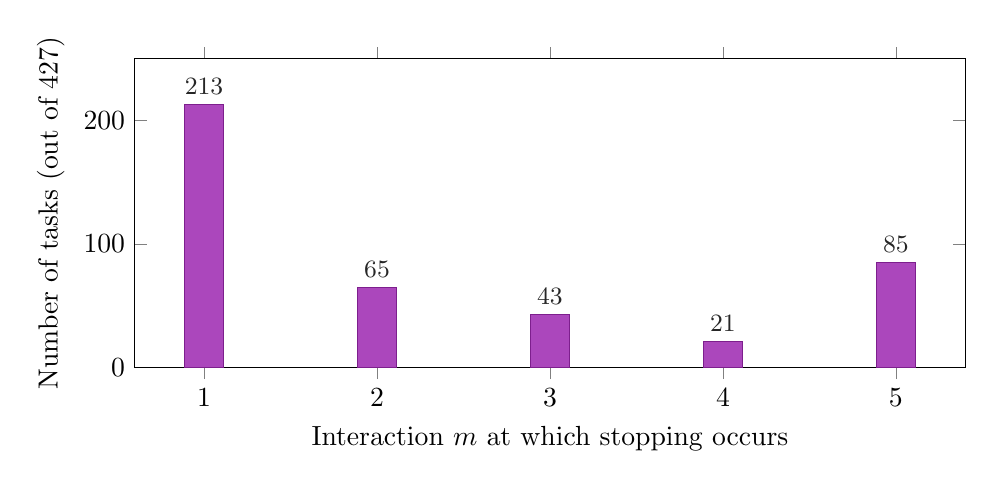
\begin{tikzpicture}
\begin{axis}[
    ybar,
    width=\columnwidth,
    height=5.5cm,
    bar width=14pt,
    xlabel={Interaction $m$ at which stopping occurs},
    ylabel={Number of tasks (out of 427)},
    ymin=0,
    ymax=250,
    xtick={1,2,3,4,5},
    nodes near coords,
    nodes near coords style={font=\small, above},
    every axis plot/.append style={fill opacity=0.85},
]
\addplot[fill=bothcolor, draw=bothcolor!80!black] coordinates {(1,213) (2,65) (3,43) (4,21) (5,85)};
\end{axis}
\end{tikzpicture}
\caption{Distribution of stopping interaction for soft scoring + entropy stopping (\textsc{PassFail}). Half of all tasks (213/427) converge after a single oracle query, while 85 tasks require the full budget of 5 interactions. The entropy criterion naturally allocates more interactions to tasks with greater behavioral diversity among candidates.}
\label{fig:efficiency}
\end{figure}

\subsection{Phase 4: Noise Robustness}

Phase~4 provides the central experimental finding. Table~\ref{tab:noise} and Figure~\ref{fig:noise} compare hard pruning and soft scoring under identical 20\% oracle noise (1 random flip per task).

\subsubsection{Hard Pruning Under Noise}

Hard pruning drops from 67.92\% (perfect oracle) to 61.83\% ($-6.09$ points) and remains \emph{completely flat} across all values of $m$. This flatness reveals a critical property: the damage occurs at the flipped interaction and is irreversible. Once the noisy oracle response causes incorrect pruning, subsequent correct interactions cannot restore the eliminated codes. The remaining candidate pool is permanently biased, and additional interactions merely rearrange an already degraded set.

\subsubsection{Soft Scoring Under Noise}

Soft scoring starts at a similar level of degradation ($m=1$: 61.59\%) but shows a distinctive recovery trajectory. By $m=2$, it recovers to 66.51\%; by $m=3$, it surpasses the \emph{perfect-oracle} Phase~2 baseline (68.62\% vs.\ 67.92\%). The final score of 68.15\% at $m=5$ represents only a $-1.17$ point loss compared to soft scoring under perfect oracle conditions (69.32\%).

The recovery mechanism is straightforward: a correct code that receives $-1$ from the noisy interaction accumulates $+1$ from the remaining 4 honest interactions, yielding a net score of $+3$. An incorrect code, by contrast, tends to receive $-1$ from multiple honest interactions, so the noisy $+1$ it may gain is insufficient to overcome its accumulated penalties.

\begin{table}[t]
\centering
\caption{Phase 4: Noise Robustness (1 random flip per task, \textsc{PassFail})}
\label{tab:noise}
\begin{tabular}{lccc}
\toprule
 & \textbf{Phase 2} & \textbf{Hard + noise} & \textbf{Soft + noise} \\
\textbf{Metric} & \textbf{(0 flips)} & \textbf{(1 flip)} & \textbf{(1 flip)} \\
\midrule
pass@1@1 & 67.21 & 61.83 & 61.59 \\
pass@1@2 & 67.92 & 61.83 & 66.51 \\
pass@1@3 & 67.92 & 61.83 & \textbf{68.62} \\
pass@1@4 & 67.92 & 61.83 & \textbf{68.62} \\
pass@1@5 & 67.92 & 61.83 & 68.15 \\
\midrule
$\Delta$ vs Phase 2 & --- & $-6.09$ & $+0.23$ \\
\bottomrule
\end{tabular}
\end{table}

\begin{figure}[t]
\centering
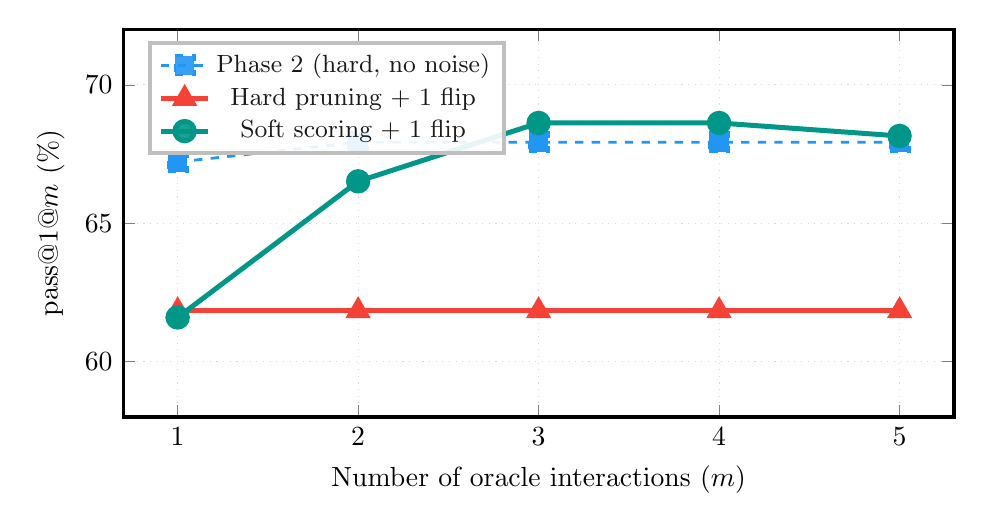
\begin{tikzpicture}
\begin{axis}[
    width=\columnwidth,
    height=6.5cm,
    xlabel={Number of oracle interactions ($m$)},
    ylabel={pass@1@$m$ (\%)},
    xmin=0.7, xmax=5.3,
    ymin=58, ymax=72,
    xtick={1,2,3,4,5},
    legend style={at={(0.03,0.97)}, anchor=north west, font=\small, fill=white, fill opacity=0.9, draw=gray!50},
    grid=major,
    grid style={dotted, gray!30},
    mark size=3.5pt,
    line width=1.3pt,
]
% Phase 2 (perfect oracle, hard pruning) - dashed reference
\addplot[color=phase2color, mark=square*, dashed, line width=1pt] coordinates {
    (1, 67.21) (2, 67.92) (3, 67.92) (4, 67.92) (5, 67.92)
};
% Hard pruning + noise - solid red, prominent
\addplot[color=hardnoisecolor, mark=triangle*, line width=1.8pt] coordinates {
    (1, 61.83) (2, 61.83) (3, 61.83) (4, 61.83) (5, 61.83)
};
% Soft scoring + noise - solid teal, prominent
\addplot[color=softnoisecolor, mark=*, line width=1.8pt] coordinates {
    (1, 61.59) (2, 66.51) (3, 68.62) (4, 68.62) (5, 68.15)
};

\legend{
    Phase 2 (hard{,} no noise),
    Hard pruning + 1 flip,
    Soft scoring + 1 flip
}
\end{axis}
\end{tikzpicture}
\caption{Noise robustness comparison (\textsc{PassFail}). The dashed blue line shows the Phase~2 reference (hard pruning, perfect oracle). Under 1 noisy flip, hard pruning (red) suffers permanent $-6.09$ point degradation that never recovers regardless of additional interactions. Soft scoring (teal) starts equally degraded but self-recovers by $m=3$, surpassing even the perfect-oracle baseline.}
\label{fig:noise}
\end{figure}

\subsection{Summary of All Configurations}

Figure~\ref{fig:summary} provides an overview of pass@1@5 across all configurations tested.

\begin{figure}[t]
\centering
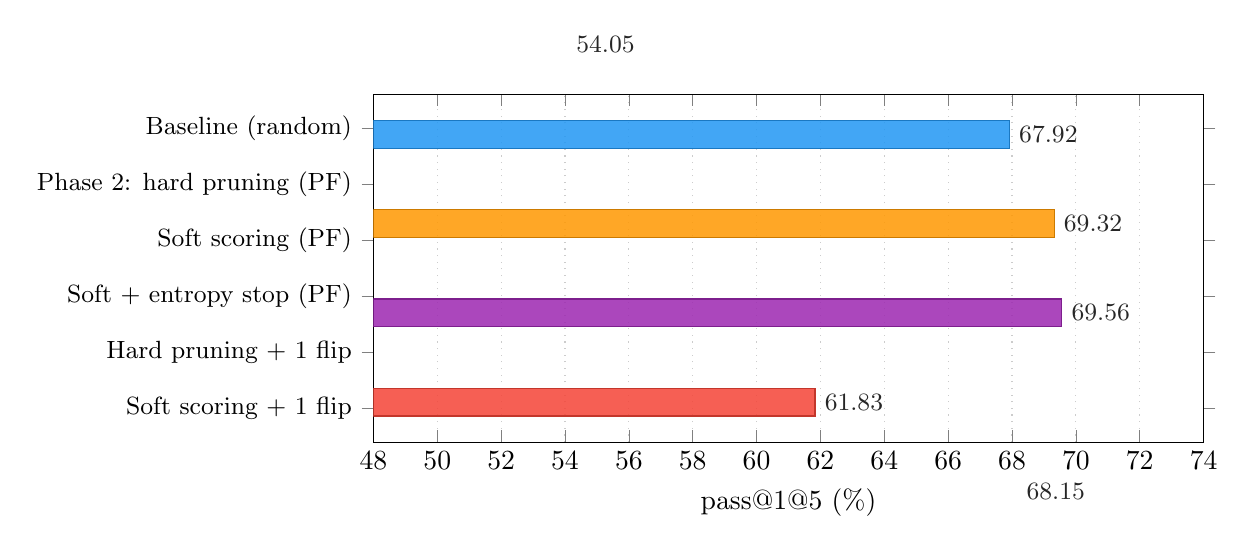
\begin{tikzpicture}
\begin{axis}[
    xbar,
    width=\columnwidth,
    height=6cm,
    bar width=10pt,
    xlabel={pass@1@5 (\%)},
    xmin=48, xmax=74,
    ytick={1,2,3,4,5,6},
    yticklabels={
        {Soft scoring + 1 flip},
        {Hard pruning + 1 flip},
        {Soft + entropy stop (PF)},
        {Soft scoring (PF)},
        {Phase 2: hard pruning (PF)},
        {Baseline (random)}
    },
    y tick label style={font=\small, anchor=east},
    nodes near coords,
    nodes near coords style={font=\small, anchor=west},
    every axis plot/.append style={fill opacity=0.85},
    xmajorgrids=true,
    grid style={dotted, gray!40},
    enlarge y limits={abs=0.6},
]
\addplot[fill=softnoisecolor, draw=softnoisecolor!80!black] coordinates {(68.15, 1)};
\addplot[fill=hardnoisecolor, draw=hardnoisecolor!80!black] coordinates {(61.83, 2)};
\addplot[fill=bothcolor, draw=bothcolor!80!black] coordinates {(69.56, 3)};
\addplot[fill=tool2color, draw=tool2color!80!black] coordinates {(69.32, 4)};
\addplot[fill=phase2color, draw=phase2color!80!black] coordinates {(67.92, 5)};
\addplot[fill=gray!60, draw=gray!80!black] coordinates {(54.05, 6)};
\end{axis}
\end{tikzpicture}
\caption{Summary of pass@1@5 across all configurations (\textsc{PassFail}). Soft scoring with entropy stopping achieves the highest perfect-oracle score (69.56\%). Under noise, soft scoring (68.15\%) vastly outperforms hard pruning (61.83\%), demonstrating its practical robustness advantage.}
\label{fig:summary}
\end{figure}

% ============================================================
\section{Discussion}
% ============================================================

\subsection{The Feedback Loop: Why Entropy Needs Soft Scoring}

A key insight from our work is that entropy-based stopping is only meaningful when paired with soft scoring. Under hard pruning, all surviving codes agree on every approved test by construction---disagreeing codes were already eliminated. Consequently, entropy over approved tests is trivially zero after the first oracle approval, and the stopping criterion degenerates to ``always stop after one interaction.'' This is not a useful signal.

With soft scoring, no codes are removed. After the oracle answers a question, codes that disagree are penalized but remain in the pool. Entropy then reflects \emph{genuine} behavioral diversity: if many codes still exhibit distinct execution patterns on approved tests, $H$ remains high, signaling that further interactions could productively shift the ranking. When codes converge to a single dominant behavior, $H$ drops, and the loop terminates.

This creates a natural feedback cycle: $s_{\text{discr}}$ selects the test that maximally splits codes, the oracle answers, soft scoring adjusts all scores, and entropy checks whether the answer resolved the uncertainty. If it did, we stop. If not, we select the next most discriminative test.

The 54\% savings in oracle calls has direct practical implications. In human-in-the-loop scenarios where each oracle query requires a developer to evaluate a test case, reducing from 5 to 2.3 interactions on average saves significant time. For automated oracles (e.g., execution-based testing), the savings translate to reduced compute costs and faster iteration cycles.

\subsection{Soft Scoring: Accuracy vs.\ Robustness}

Soft scoring presents a nuanced accuracy--robustness tradeoff that depends on the oracle variant:

\textbf{Under \textsc{PassFail}:} Soft scoring is strictly beneficial, improving accuracy by +1.63 points at $m=5$. The advantage likely stems from soft scoring's ability to accumulate evidence across multiple tests, whereas hard pruning's binary decisions can be overly aggressive---correct codes that happen to fail one test (e.g., due to edge case handling differences) are permanently lost.

\textbf{Under \textsc{Output}:} Hard pruning retains a 0.94-point advantage because the \textsc{Output} oracle provides precise output-level information that hard pruning can fully exploit. Soft scoring's $\pm 1$ granularity collapses this rich signal into a binary agree/disagree, losing discriminative power. A potential improvement would be to weight $\delta$ by the specificity of the oracle's response, assigning larger magnitudes when output information is available.

\textbf{Under noise:} Soft scoring's advantage becomes dramatic. The 6.32-point gap between soft scoring and hard pruning under noise (68.15\% vs.\ 61.83\%) far exceeds the 0.94-point cost under the best-case \textsc{Output} scenario with a perfect oracle. In any deployment where oracle noise is a possibility---which is nearly all practical scenarios---soft scoring is the safer choice.

\subsection{Why Hard Pruning Flatlines Under Noise}

The constant 61.83\% across all $m$ values for noisy hard pruning (Figure~\ref{fig:noise}) demands explanation. When a noisy oracle incorrectly responds FAIL for a test that the reference code actually passes, hard pruning removes all surviving codes that pass that test. Since correct codes are more likely to pass the test (they implement the correct behavior), this disproportionately eliminates correct candidates.

The safety fallback in our implementation---keeping all codes when pruning would eliminate every candidate---prevents catastrophic failure (0\% accuracy) but cannot undo selective damage. The surviving pool is biased toward codes that happened to fail the noisy test, and no amount of additional correct interactions can reintroduce the pruned candidates.

This is a structural limitation of any pruning-based approach: \emph{information destroyed by incorrect pruning cannot be recovered}. Soft scoring avoids this by treating each interaction as evidence that adjusts scores rather than gates that eliminate candidates.

\subsection{Entropy Stopping Prevents Over-Interaction}

An interesting detail emerges from comparing soft scoring with and without entropy stopping: at $m=5$, soft scoring alone regresses slightly (69.56\% at $m=4$ $\to$ 69.32\% at $m=5$), while the combined approach maintains 69.56\% at $m=5$. This occurs because entropy stopping locks in the peak ranking at $m=4$ for tasks that have already converged. Without it, the fifth interaction can introduce minor perturbations that slightly degrade an already-optimal ranking.

This demonstrates that entropy stopping is not merely an efficiency optimization---it also serves as a \emph{quality preservation} mechanism, preventing unnecessary interactions from perturbing a stabilized ranking.

% ============================================================
\section{Threats to Validity}
% ============================================================

\textbf{Single model.} Our experiments use only Claude Haiku. Models with different code generation characteristics (e.g., higher diversity or accuracy) may interact differently with our tools. However, the underlying mechanisms---entropy convergence and score accumulation---are model-agnostic.

\textbf{Single benchmark.} MBPP tasks are relatively simple Python functions (typically 2--15 lines). More complex benchmarks such as HumanEval+~\cite{liu2023humaneval}, APPS~\cite{hendrycks2021apps}, or SWE-bench~\cite{jimenez2024swebench} may present different interaction dynamics. In particular, complex tasks may require more interactions before entropy converges, potentially reducing the efficiency gains of early stopping.

\textbf{Simplified noise model.} Our noise injection uses uniform random single flips, which is a simplified model of real-world oracle errors. Practical noise may be correlated with task difficulty (harder tasks elicit more oracle errors) or test quality (ambiguous tests are more likely to produce incorrect responses). Evaluating under such structured noise patterns is an important direction for future work.

\textbf{Fixed hyperparameters.} The entropy threshold ($\tau = 0.5$) and soft scoring weights ($\pm 1$) were not tuned via validation. The threshold was chosen based on the intuition that $H < 0.5$ indicates a dominant cluster, but systematic tuning could yield better results. Similarly, the uniform $\pm 1$ weighting could be replaced with confidence-weighted scores based on test discriminative power.

\textbf{Oracle simulation.} We use the reference solution as a simulated oracle, which may not capture the full complexity of human oracle behavior (e.g., partial understanding, inconsistent responses across similar tests).

% ============================================================
\section{Future Work}
% ============================================================

Several extensions could build on our results:

\textbf{Weighted soft scoring.} Instead of uniform $\pm 1$ weights, assign larger magnitudes to tests with higher discriminative scores ($s_{\text{discr}}$) or to responses that include output-level information. This could recover the \textsc{Output} variant's advantage while retaining noise resilience.

\textbf{Adaptive entropy threshold.} Rather than a fixed $\tau = 0.5$, the threshold could be adapted based on the number of candidates, task complexity, or the rate of entropy change across interactions.

\textbf{Hybrid pruning.} Combine soft scoring with selective hard pruning: use soft scoring by default, but apply hard pruning when oracle confidence is high (e.g., when the oracle provides specific output values). This could capture the strengths of both approaches.

\textbf{Multi-model evaluation.} Extend the evaluation to additional code generation models (GPT-4, CodeLlama, DeepSeek-Coder) and benchmarks (HumanEval+, APPS) to assess generalizability.

\textbf{Realistic noise models.} Evaluate under structured noise that correlates with task or test properties, and explore online noise detection as an additional tool.

% ============================================================
\section{Conclusion}
% ============================================================

We presented an integrated extension to TICODER comprising soft scoring and entropy-based early stopping, forming a unified feedback loop for interactive code generation. The discriminative metric selects the most informative test, the oracle answers, soft scoring accumulates the evidence, and entropy checks whether the uncertainty has been resolved. This loop naturally adapts its interaction budget to each task's difficulty, achieving 69.56\% pass@1@5 on MBPP while requiring only 2.3 interactions on average---a 54\% reduction in oracle calls.

The noise robustness experiment provides the strongest motivation for adoption: under 20\% oracle noise, hard pruning suffers a permanent $-6.09$ point degradation with no recovery path, while soft scoring limits the damage to $-1.17$ points and self-corrects by the third interaction. The 6.32-point advantage under noise far outweighs the 0.94-point cost under perfect \textsc{Output} oracle conditions.

Crucially, entropy-based stopping is only meaningful with soft scoring---under hard pruning, survivors trivially agree on all approved tests, making entropy uninformative. Together, these components transform TICODER from a system that is optimal but fragile into one that is robust and efficient, suitable for practical deployments where oracle feedback may be imperfect.

\balance

\bibliographystyle{IEEEtran}
\begin{thebibliography}{10}

\bibitem{ticoder}
H.~Lahiri, S.~Fakhoury, A.~Naik, G.~Musuvathi, and S.~K.~Rajamani,
``Interactive code generation via test-driven user-intent formalization,''
\textit{arXiv preprint arXiv:2404.10882}, 2024.

\bibitem{chen2021codex}
M.~Chen, J.~Tworek, H.~Jun, Q.~Yuan, H.~Pinto de Oliveira, J.~Kaplan, et~al.,
``Evaluating large language models trained on code,''
\textit{arXiv preprint arXiv:2107.03374}, 2021.

\bibitem{li2023starcoder}
R.~Li, L.~B.~Allal, Y.~Zi, N.~Muennighoff, D.~Kocetkov, et~al.,
``StarCoder: may the source be with you!''
\textit{arXiv preprint arXiv:2305.06161}, 2023.

\bibitem{roziere2023codellama}
B.~Rozi\`{e}re, J.~Gehring, F.~Gloeckle, S.~Sootla, I.~Gat, et~al.,
``Code Llama: Open foundation models for code,''
\textit{arXiv preprint arXiv:2308.12950}, 2023.

\bibitem{austin2021mbpp}
J.~Austin, A.~Odena, M.~Nye, M.~Bosma, H.~Michalewski, et~al.,
``Program synthesis with large language models,''
\textit{arXiv preprint arXiv:2108.07732}, 2021.

\bibitem{chen2022codet}
B.~Chen, F.~Zhang, A.~Nguyen, D.~Zan, Z.~Lin, J.-G.~Lou, and W.~Chen,
``CodeT: Code generation with generated tests,''
\textit{arXiv preprint arXiv:2207.10397}, 2022.

\bibitem{shi2022mbr}
F.~Shi, D.~Fried, M.~Ghazvininejad, L.~Zettlemoyer, and S.~I.~Wang,
``Natural language to code translation with execution,''
\textit{arXiv preprint arXiv:2204.11454}, 2022.

\bibitem{liu2023humaneval}
J.~Liu, C.~S.~Xia, Y.~Wang, and L.~Zhang,
``Is your code generated by ChatGPT really correct? Rigorous evaluation of large language models for code generation,''
\textit{NeurIPS}, 2023.

\bibitem{hendrycks2021apps}
D.~Hendrycks, S.~Basart, S.~Kadavath, M.~Mazeika, A.~Arora, et~al.,
``Measuring coding challenge competence with APPS,''
\textit{NeurIPS}, 2021.

\bibitem{jimenez2024swebench}
C.~E.~Jimenez, J.~Yang, A.~Wettig, S.~Yao, K.~Pei, O.~Press, and K.~Narasimhan,
``SWE-bench: Can language models resolve real-world GitHub issues?''
\textit{ICLR}, 2024.

\end{thebibliography}

\end{document}
